\documentclass[]{book}
\usepackage{lmodern}
\usepackage{amssymb,amsmath}
\usepackage{ifxetex,ifluatex}
\usepackage{fixltx2e} % provides \textsubscript
\ifnum 0\ifxetex 1\fi\ifluatex 1\fi=0 % if pdftex
  \usepackage[T1]{fontenc}
  \usepackage[utf8]{inputenc}
\else % if luatex or xelatex
  \ifxetex
    \usepackage{mathspec}
  \else
    \usepackage{fontspec}
  \fi
  \defaultfontfeatures{Ligatures=TeX,Scale=MatchLowercase}
\fi
% use upquote if available, for straight quotes in verbatim environments
\IfFileExists{upquote.sty}{\usepackage{upquote}}{}
% use microtype if available
\IfFileExists{microtype.sty}{%
\usepackage{microtype}
\UseMicrotypeSet[protrusion]{basicmath} % disable protrusion for tt fonts
}{}
\usepackage[margin=1in]{geometry}
\usepackage{hyperref}
\hypersetup{unicode=true,
            pdftitle={R Advanced Spatial Lessons},
            pdfauthor={Ben Best},
            pdfborder={0 0 0},
            breaklinks=true}
\urlstyle{same}  % don't use monospace font for urls
\usepackage{color}
\usepackage{fancyvrb}
\newcommand{\VerbBar}{|}
\newcommand{\VERB}{\Verb[commandchars=\\\{\}]}
\DefineVerbatimEnvironment{Highlighting}{Verbatim}{commandchars=\\\{\}}
% Add ',fontsize=\small' for more characters per line
\usepackage{framed}
\definecolor{shadecolor}{RGB}{248,248,248}
\newenvironment{Shaded}{\begin{snugshade}}{\end{snugshade}}
\newcommand{\KeywordTok}[1]{\textcolor[rgb]{0.13,0.29,0.53}{\textbf{{#1}}}}
\newcommand{\DataTypeTok}[1]{\textcolor[rgb]{0.13,0.29,0.53}{{#1}}}
\newcommand{\DecValTok}[1]{\textcolor[rgb]{0.00,0.00,0.81}{{#1}}}
\newcommand{\BaseNTok}[1]{\textcolor[rgb]{0.00,0.00,0.81}{{#1}}}
\newcommand{\FloatTok}[1]{\textcolor[rgb]{0.00,0.00,0.81}{{#1}}}
\newcommand{\ConstantTok}[1]{\textcolor[rgb]{0.00,0.00,0.00}{{#1}}}
\newcommand{\CharTok}[1]{\textcolor[rgb]{0.31,0.60,0.02}{{#1}}}
\newcommand{\SpecialCharTok}[1]{\textcolor[rgb]{0.00,0.00,0.00}{{#1}}}
\newcommand{\StringTok}[1]{\textcolor[rgb]{0.31,0.60,0.02}{{#1}}}
\newcommand{\VerbatimStringTok}[1]{\textcolor[rgb]{0.31,0.60,0.02}{{#1}}}
\newcommand{\SpecialStringTok}[1]{\textcolor[rgb]{0.31,0.60,0.02}{{#1}}}
\newcommand{\ImportTok}[1]{{#1}}
\newcommand{\CommentTok}[1]{\textcolor[rgb]{0.56,0.35,0.01}{\textit{{#1}}}}
\newcommand{\DocumentationTok}[1]{\textcolor[rgb]{0.56,0.35,0.01}{\textbf{\textit{{#1}}}}}
\newcommand{\AnnotationTok}[1]{\textcolor[rgb]{0.56,0.35,0.01}{\textbf{\textit{{#1}}}}}
\newcommand{\CommentVarTok}[1]{\textcolor[rgb]{0.56,0.35,0.01}{\textbf{\textit{{#1}}}}}
\newcommand{\OtherTok}[1]{\textcolor[rgb]{0.56,0.35,0.01}{{#1}}}
\newcommand{\FunctionTok}[1]{\textcolor[rgb]{0.00,0.00,0.00}{{#1}}}
\newcommand{\VariableTok}[1]{\textcolor[rgb]{0.00,0.00,0.00}{{#1}}}
\newcommand{\ControlFlowTok}[1]{\textcolor[rgb]{0.13,0.29,0.53}{\textbf{{#1}}}}
\newcommand{\OperatorTok}[1]{\textcolor[rgb]{0.81,0.36,0.00}{\textbf{{#1}}}}
\newcommand{\BuiltInTok}[1]{{#1}}
\newcommand{\ExtensionTok}[1]{{#1}}
\newcommand{\PreprocessorTok}[1]{\textcolor[rgb]{0.56,0.35,0.01}{\textit{{#1}}}}
\newcommand{\AttributeTok}[1]{\textcolor[rgb]{0.77,0.63,0.00}{{#1}}}
\newcommand{\RegionMarkerTok}[1]{{#1}}
\newcommand{\InformationTok}[1]{\textcolor[rgb]{0.56,0.35,0.01}{\textbf{\textit{{#1}}}}}
\newcommand{\WarningTok}[1]{\textcolor[rgb]{0.56,0.35,0.01}{\textbf{\textit{{#1}}}}}
\newcommand{\AlertTok}[1]{\textcolor[rgb]{0.94,0.16,0.16}{{#1}}}
\newcommand{\ErrorTok}[1]{\textcolor[rgb]{0.64,0.00,0.00}{\textbf{{#1}}}}
\newcommand{\NormalTok}[1]{{#1}}
\usepackage{longtable,booktabs}
\usepackage{graphicx,grffile}
\makeatletter
\def\maxwidth{\ifdim\Gin@nat@width>\linewidth\linewidth\else\Gin@nat@width\fi}
\def\maxheight{\ifdim\Gin@nat@height>\textheight\textheight\else\Gin@nat@height\fi}
\makeatother
% Scale images if necessary, so that they will not overflow the page
% margins by default, and it is still possible to overwrite the defaults
% using explicit options in \includegraphics[width, height, ...]{}
\setkeys{Gin}{width=\maxwidth,height=\maxheight,keepaspectratio}
\IfFileExists{parskip.sty}{%
\usepackage{parskip}
}{% else
\setlength{\parindent}{0pt}
\setlength{\parskip}{6pt plus 2pt minus 1pt}
}
\setlength{\emergencystretch}{3em}  % prevent overfull lines
\providecommand{\tightlist}{%
  \setlength{\itemsep}{0pt}\setlength{\parskip}{0pt}}
\setcounter{secnumdepth}{5}
% Redefines (sub)paragraphs to behave more like sections
\ifx\paragraph\undefined\else
\let\oldparagraph\paragraph
\renewcommand{\paragraph}[1]{\oldparagraph{#1}\mbox{}}
\fi
\ifx\subparagraph\undefined\else
\let\oldsubparagraph\subparagraph
\renewcommand{\subparagraph}[1]{\oldsubparagraph{#1}\mbox{}}
\fi

%%% Use protect on footnotes to avoid problems with footnotes in titles
\let\rmarkdownfootnote\footnote%
\def\footnote{\protect\rmarkdownfootnote}

%%% Change title format to be more compact
\usepackage{titling}

% Create subtitle command for use in maketitle
\newcommand{\subtitle}[1]{
  \posttitle{
    \begin{center}\large#1\end{center}
    }
}

\setlength{\droptitle}{-2em}
  \title{R Advanced Spatial Lessons}
  \pretitle{\vspace{\droptitle}\centering\huge}
  \posttitle{\par}
  \author{Ben Best}
  \preauthor{\centering\large\emph}
  \postauthor{\par}
  \predate{\centering\large\emph}
  \postdate{\par}
  \date{2017-09-24}

\usepackage{booktabs}
\usepackage{amsthm}
\makeatletter
\def\thm@space@setup{%
  \thm@preskip=8pt plus 2pt minus 4pt
  \thm@postskip=\thm@preskip
}
\makeatother

\begin{document}
\maketitle

{
\setcounter{tocdepth}{1}
\tableofcontents
}
\chapter*{Prerequisites}\label{prereq}
\addcontentsline{toc}{chapter}{Prerequisites}

Lessons presented here are a continuation of the
\href{http://www.datacarpentry.org/lessons/\#geospatial-data-workshop}{Geospatial
workshop using R of Data Carpentry} described more specifically for the
\href{https://jsta.github.io/2017-09-27-LBNL/}{Lawrence Berkeley
National Lab: Sep 27-28, 2017}.

This content is setup for now using
\href{http://bookdown.org/yihui/bookdown}{bookdown} (using the
\href{https://github.com/rstudio/bookdown-demo}{bookdown-demo}) for
expediency, and meant to eventually be folded into the
\href{https://github.com/swcarpentry/styles}{Software Carpentry style}.

\chapter{Tidy Spatial Analysis}\label{tidy}

Resources:

\begin{itemize}
\tightlist
\item
  \href{http://strimas.com/r/tidy-sf/}{Tidy spatial data in R: using
  dplyr, tidyr, and ggplot2 with sf}
\end{itemize}

\section{Overview}\label{overview}

\textbf{Questions} - How to elegantly conduct complex spatial analysis?

\textbf{Objectives} - Use the \texttt{\%\textgreater{}\%} operator (aka
``then'' or ``pipe'') to pass output from one function into input of the
next. - Calculate metrics on spatial attributes. - Aggregate spatial
data with metrics.

\section{Things You'll Need to Complete this
Tutorial}\label{things-youll-need-to-complete-this-tutorial}

\textbf{R Skill Level}: Intermediate - you've got basics of R down.

You'll need \ldots{}

We will use the \texttt{sf} package for vector data along with the
\texttt{dplyr} package for calculating and manipulating attribute data.

\begin{Shaded}
\begin{Highlighting}[]
\CommentTok{# load packages}
\KeywordTok{library}\NormalTok{(tidyverse)  }\CommentTok{# dplyr, tidyr, ggplot2}
\KeywordTok{library}\NormalTok{(sf)         }\CommentTok{# vector reading & analysis}

\CommentTok{# set working directory to data folder}
\CommentTok{# setwd("pathToDirHere")}
\end{Highlighting}
\end{Shaded}

\section{US States: Read and Plot}\label{us-states-read-and-plot}

Similar to
\href{https://jsta.github.io/R-spatial-raster-vector-lesson/09-vector-when-data-dont-line-up-crs/}{Lesson
9: Handling Spatial Projection \& CRS in R}, we'll start by reading in a
polygon shapefile using the \texttt{sf} package. Then use the default
\texttt{plot()} function to see what it looks like.

\begin{Shaded}
\begin{Highlighting}[]
\CommentTok{# read in states}
\NormalTok{states <-}\StringTok{ }\KeywordTok{read_sf}\NormalTok{(}\StringTok{"data/NEON-DS-Site-Layout-Files/US-Boundary-Layers/US-State-Boundaries-Census-2014.shp"}\NormalTok{)}
\KeywordTok{plot}\NormalTok{(states)}
\end{Highlighting}
\end{Shaded}

\begin{verbatim}
## Warning: plotting the first 9 out of 10 attributes; use max.plot = 10 to
## plot all
\end{verbatim}

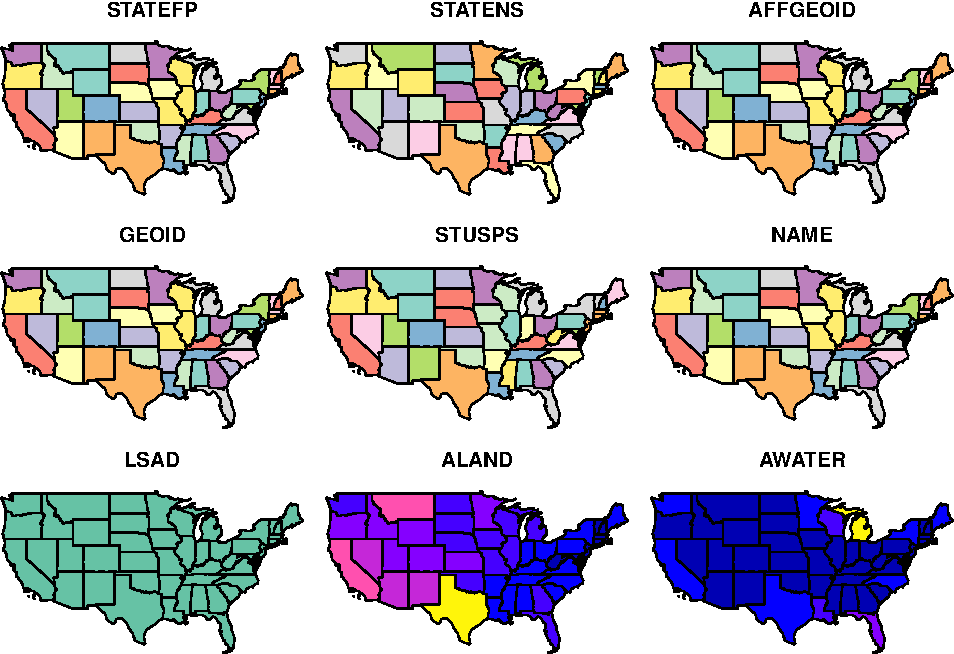
\includegraphics{R-adv-spatial_files/figure-latex/unnamed-chunk-2-1.pdf}

You'll notice that the default plot on \texttt{sf} objects outputs
colorized values of the first 9 of 10 columns. Use the suggestion from
the warning to plot the 10th column.

\begin{Shaded}
\begin{Highlighting}[]
\CommentTok{# plot 10th column}
\KeywordTok{plot}\NormalTok{(states, }\DataTypeTok{max.plot =} \DecValTok{10}\NormalTok{)}
\end{Highlighting}
\end{Shaded}

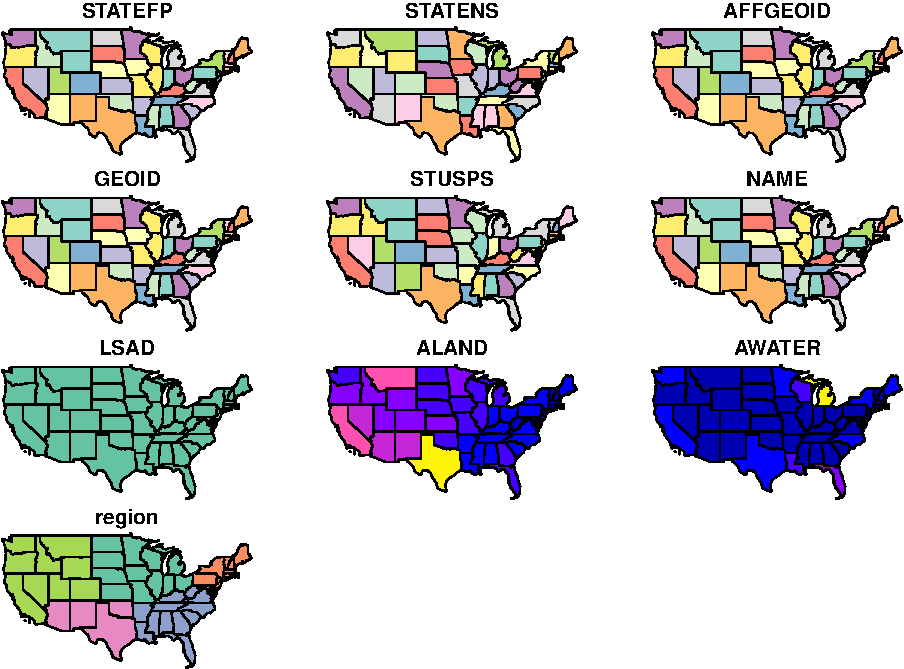
\includegraphics{R-adv-spatial_files/figure-latex/unnamed-chunk-3-1.pdf}

\begin{Shaded}
\begin{Highlighting}[]
\CommentTok{# show columns of the data frame}
\KeywordTok{names}\NormalTok{(states)}
\end{Highlighting}
\end{Shaded}

\begin{verbatim}
##  [1] "STATEFP"  "STATENS"  "AFFGEOID" "GEOID"    "STUSPS"   "NAME"    
##  [7] "LSAD"     "ALAND"    "AWATER"   "region"   "geometry"
\end{verbatim}

\begin{Shaded}
\begin{Highlighting}[]
\CommentTok{# look at table}
\KeywordTok{glimpse}\NormalTok{(states)}
\end{Highlighting}
\end{Shaded}

\begin{verbatim}
## Observations: 58
## Variables: 11
## $ STATEFP  <chr> "06", "11", "12", "13", "16", "17", "19", "21", "22",...
## $ STATENS  <chr> "01779778", "01702382", "00294478", "01705317", "0177...
## $ AFFGEOID <chr> "0400000US06", "0400000US11", "0400000US12", "0400000...
## $ GEOID    <chr> "06", "11", "12", "13", "16", "17", "19", "21", "22",...
## $ STUSPS   <chr> "CA", "DC", "FL", "GA", "ID", "IL", "IA", "KY", "LA",...
## $ NAME     <chr> "California", "District of Columbia", "Florida", "Geo...
## $ LSAD     <chr> "00", "00", "00", "00", "00", "00", "00", "00", "00",...
## $ ALAND    <dbl> 403483823181, 158350578, 138903200855, 148963503399, ...
## $ AWATER   <dbl> 20483271881, 18633500, 31407883551, 4947080103, 23977...
## $ region   <chr> "West", "Northeast", "Southeast", "Southeast", "West"...
## $ geometry <simple_feature> MULTIPOLYGONZ(((-118.593969..., MULTIPOLYG...
\end{verbatim}

\begin{Shaded}
\begin{Highlighting}[]
\CommentTok{# convert to tibble for nicer printing}
\KeywordTok{as_tibble}\NormalTok{(states)}
\end{Highlighting}
\end{Shaded}

\begin{verbatim}
## Simple feature collection with 58 features and 10 fields
## geometry type:  MULTIPOLYGON
## dimension:      XYZ
## bbox:           xmin: -124.7258 ymin: 24.49813 xmax: -66.9499 ymax: 49.38436
## epsg (SRID):    4326
## proj4string:    +proj=longlat +datum=WGS84 +no_defs
## # A tibble: 58 x 11
##    STATEFP  STATENS    AFFGEOID GEOID STUSPS                 NAME  LSAD
##      <chr>    <chr>       <chr> <chr>  <chr>                <chr> <chr>
##  1      06 01779778 0400000US06    06     CA           California    00
##  2      11 01702382 0400000US11    11     DC District of Columbia    00
##  3      12 00294478 0400000US12    12     FL              Florida    00
##  4      13 01705317 0400000US13    13     GA              Georgia    00
##  5      16 01779783 0400000US16    16     ID                Idaho    00
##  6      17 01779784 0400000US17    17     IL             Illinois    00
##  7      19 01779785 0400000US19    19     IA                 Iowa    00
##  8      21 01779786 0400000US21    21     KY             Kentucky    00
##  9      22 01629543 0400000US22    22     LA            Louisiana    00
## 10      24 01714934 0400000US24    24     MD             Maryland    00
## # ... with 48 more rows, and 4 more variables: ALAND <dbl>, AWATER <dbl>,
## #   region <chr>, geometry <simple_feature>
\end{verbatim}

\begin{Shaded}
\begin{Highlighting}[]
\KeywordTok{names}\NormalTok{(states)}
\end{Highlighting}
\end{Shaded}

\begin{verbatim}
##  [1] "STATEFP"  "STATENS"  "AFFGEOID" "GEOID"    "STUSPS"   "NAME"    
##  [7] "LSAD"     "ALAND"    "AWATER"   "region"   "geometry"
\end{verbatim}

\begin{Shaded}
\begin{Highlighting}[]
\CommentTok{# inspect the class(es) of the states object}
\KeywordTok{class}\NormalTok{(states)}
\end{Highlighting}
\end{Shaded}

\begin{verbatim}
## [1] "sf"         "tbl_df"     "tbl"        "data.frame"
\end{verbatim}

The class of the \texttt{states} object is both a simple feature
(\texttt{sf}) as well as a data frame, which means the many useful
functions available to a data frame (or ``tibble'') can be applied.

To plot the column of interest, feed the ``slice'' of that column to the
\texttt{plot()} function.

\begin{Shaded}
\begin{Highlighting}[]
\KeywordTok{plot}\NormalTok{(states[}\StringTok{'region'}\NormalTok{])}
\end{Highlighting}
\end{Shaded}

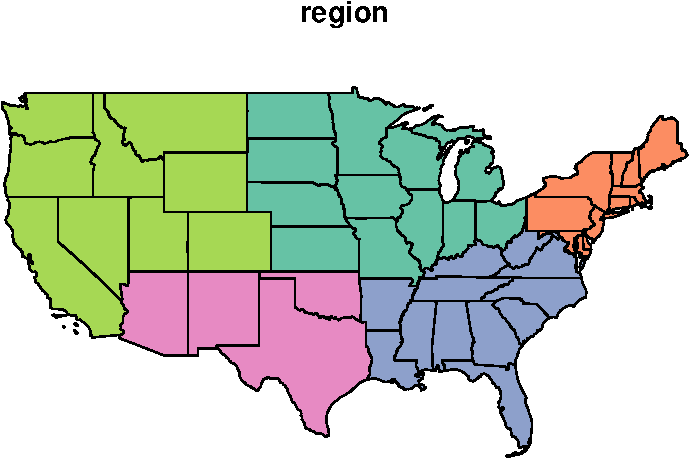
\includegraphics{R-adv-spatial_files/figure-latex/unnamed-chunk-4-1.pdf}

\textbf{Question}: To motivate the spatial analysis for the rest of this
lesson, let's answer this question: ``\emph{\textbf{Show which regions
have the highest ratio of water to land?}}''

\section{Challenge: What analytical steps are required to answer the
question?}\label{challenge-what-analytical-steps-are-required-to-answer-the-question}

Outline a sequence of analytical steps needed to arrive at the answer.

\subsection{Answers}\label{answers}

\begin{enumerate}
\def\labelenumi{\arabic{enumi}.}
\tightlist
\item
  \textbf{Sum} the area of water and land per region.
\item
  \textbf{Divide} the area of water by the area of land per region to
  arrive at density of water.
\item
  Show \textbf{table} of regions sorted by density of water.
\item
  Show \textbf{map} of regions by density of water with a color ramp and
  legend.
\end{enumerate}

\section{US States: Analyze
Attributes}\label{us-states-analyze-attributes}

\begin{Shaded}
\begin{Highlighting}[]
\NormalTok{regions =}\StringTok{ }\NormalTok{states %>%}
\StringTok{  }\KeywordTok{group_by}\NormalTok{(region) %>%}
\StringTok{  }\KeywordTok{summarize}\NormalTok{(}
    \DataTypeTok{water =} \KeywordTok{sum}\NormalTok{(AWATER),}
    \DataTypeTok{land  =} \KeywordTok{sum}\NormalTok{(ALAND)) %>%}
\StringTok{  }\KeywordTok{mutate}\NormalTok{(}
    \DataTypeTok{water_land =} \NormalTok{water /}\StringTok{ }\NormalTok{land)}

\CommentTok{# object}
\NormalTok{regions}
\end{Highlighting}
\end{Shaded}

\begin{verbatim}
## Simple feature collection with 5 features and 4 fields
## geometry type:  GEOMETRY
## dimension:      XYZ
## bbox:           xmin: -124.7258 ymin: 24.49813 xmax: -66.9499 ymax: 49.38436
## epsg (SRID):    4326
## proj4string:    +proj=longlat +datum=WGS84 +no_defs
## # A tibble: 5 x 5
##      region        water         land water_land          geometry
##       <chr>        <dbl>        <dbl>      <dbl>  <simple_feature>
## 1   Midwest 184383393833 1.943869e+12 0.09485380 <MULTIPOLYGON...>
## 2 Northeast 108922434345 8.690661e+11 0.12533273 <MULTIPOLYGON...>
## 3 Southeast 103876652998 1.364632e+12 0.07612063 <MULTIPOLYGON...>
## 4 Southwest  24217682268 1.462632e+12 0.01655761 <POLYGONZ((-9...>
## 5      West  57568049509 2.432336e+12 0.02366780 <MULTIPOLYGON...>
\end{verbatim}

\begin{Shaded}
\begin{Highlighting}[]
\CommentTok{# table}
\NormalTok{regions %>%}
\StringTok{  }\KeywordTok{st_set_geometry}\NormalTok{(}\OtherTok{NULL}\NormalTok{) %>%}
\StringTok{  }\KeywordTok{arrange}\NormalTok{(}\KeywordTok{desc}\NormalTok{(water_land))}
\end{Highlighting}
\end{Shaded}

\begin{verbatim}
## # A tibble: 5 x 4
##      region        water         land water_land
##       <chr>        <dbl>        <dbl>      <dbl>
## 1 Northeast 108922434345 8.690661e+11 0.12533273
## 2   Midwest 184383393833 1.943869e+12 0.09485380
## 3 Southeast 103876652998 1.364632e+12 0.07612063
## 4      West  57568049509 2.432336e+12 0.02366780
## 5 Southwest  24217682268 1.462632e+12 0.01655761
\end{verbatim}

\begin{Shaded}
\begin{Highlighting}[]
\CommentTok{# plot, default}
\KeywordTok{plot}\NormalTok{(regions[}\StringTok{'water_land'}\NormalTok{])}
\end{Highlighting}
\end{Shaded}

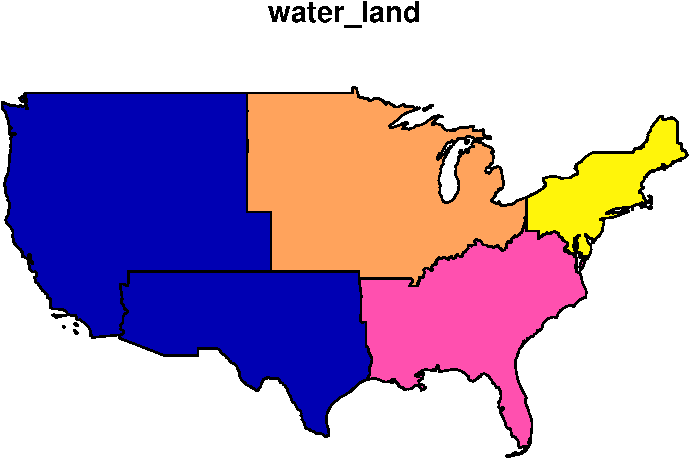
\includegraphics{R-adv-spatial_files/figure-latex/unnamed-chunk-5-1.pdf}

\begin{Shaded}
\begin{Highlighting}[]
\CommentTok{# plot, ggplot}
\KeywordTok{ggplot}\NormalTok{(regions) +}
\StringTok{  }\KeywordTok{geom_sf}\NormalTok{(}\KeywordTok{aes}\NormalTok{(}\DataTypeTok{fill =} \NormalTok{water_land)) +}
\StringTok{  }\KeywordTok{scale_fill_distiller}\NormalTok{(}\StringTok{"water_land"}\NormalTok{, }\DataTypeTok{palette =} \StringTok{"Spectral"}\NormalTok{) +}
\StringTok{  }\KeywordTok{theme_bw}\NormalTok{() +}
\StringTok{  }\KeywordTok{ggtitle}\NormalTok{(}\StringTok{"Ratio of Water to Land for US Regions"}\NormalTok{)}
\end{Highlighting}
\end{Shaded}

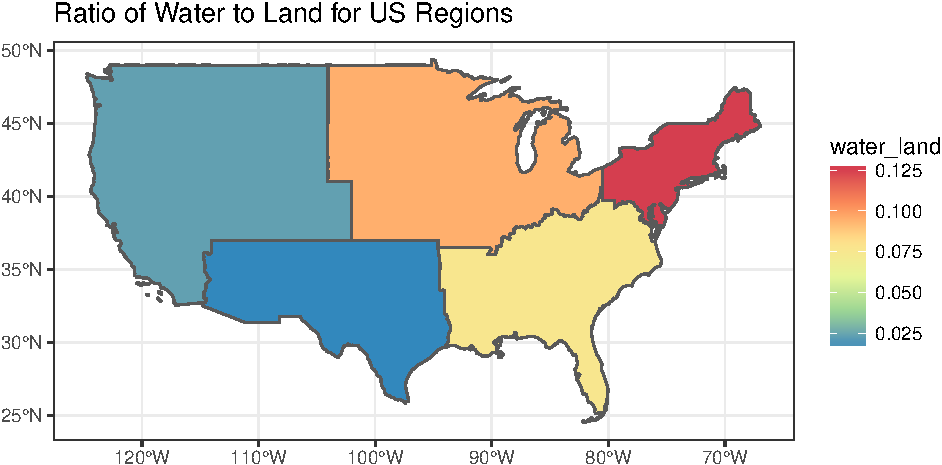
\includegraphics{R-adv-spatial_files/figure-latex/unnamed-chunk-5-2.pdf}

\section{US States: Recalculate Area}\label{us-states-recalculate-area}

Because in geographic coordinates, need to either transform to
projection and calculate area, or use geodesic calculations.

\begin{Shaded}
\begin{Highlighting}[]
\KeywordTok{library}\NormalTok{(geosphere)}
\KeywordTok{library}\NormalTok{(units)}

\NormalTok{regions =}\StringTok{ }\NormalTok{states %>%}
\StringTok{  }\KeywordTok{mutate}\NormalTok{(}
    \DataTypeTok{water_m2 =} \NormalTok{AWATER %>%}\StringTok{ }\KeywordTok{set_units}\NormalTok{(m^}\DecValTok{2}\NormalTok{),}
    \DataTypeTok{land_m2  =} \NormalTok{geometry %>%}\StringTok{ }\KeywordTok{st_zm}\NormalTok{() %>%}\StringTok{ }\KeywordTok{st_area}\NormalTok{()) %>%}
\StringTok{  }\KeywordTok{group_by}\NormalTok{(region) %>%}
\StringTok{  }\KeywordTok{summarize}\NormalTok{(}
    \DataTypeTok{water_m2 =} \KeywordTok{sum}\NormalTok{(water_m2),}
    \DataTypeTok{land_m2  =} \KeywordTok{sum}\NormalTok{(land_m2)) %>%}
\StringTok{  }\KeywordTok{mutate}\NormalTok{(}
    \DataTypeTok{water_land =} \NormalTok{water_m2 /}\StringTok{ }\NormalTok{land_m2)}

\CommentTok{# table}
\NormalTok{regions %>%}
\StringTok{  }\KeywordTok{st_set_geometry}\NormalTok{(}\OtherTok{NULL}\NormalTok{) %>%}
\StringTok{  }\KeywordTok{arrange}\NormalTok{(}\KeywordTok{desc}\NormalTok{(water_land))}
\end{Highlighting}
\end{Shaded}

\begin{verbatim}
## # A tibble: 5 x 4
##      region         water_m2          land_m2   water_land
##       <chr>          <units>          <units>      <units>
## 1 Northeast 108922434345 m^2 9.117041e+11 m^2 0.11947126 1
## 2   Midwest 184383393833 m^2 1.987268e+12 m^2 0.09278233 1
## 3 Southeast 103876652998 m^2 1.427079e+12 m^2 0.07278971 1
## 4      West  57568049509 m^2 2.467170e+12 m^2 0.02333363 1
## 5 Southwest  24217682268 m^2 1.483765e+12 m^2 0.01632178 1
\end{verbatim}

\begin{Shaded}
\begin{Highlighting}[]
\CommentTok{# plot, ggplot}
\KeywordTok{ggplot}\NormalTok{(regions) +}
\StringTok{  }\KeywordTok{geom_sf}\NormalTok{(}\KeywordTok{aes}\NormalTok{(}\DataTypeTok{fill =} \KeywordTok{as.numeric}\NormalTok{(water_land))) +}
\StringTok{  }\KeywordTok{scale_fill_distiller}\NormalTok{(}\StringTok{"water_land"}\NormalTok{, }\DataTypeTok{palette =} \StringTok{"Spectral"}\NormalTok{) +}
\StringTok{  }\KeywordTok{theme_bw}\NormalTok{() +}
\StringTok{  }\KeywordTok{ggtitle}\NormalTok{(}\StringTok{"Ratio of Water to Land (geodesic) for US Regions "}\NormalTok{)}
\end{Highlighting}
\end{Shaded}

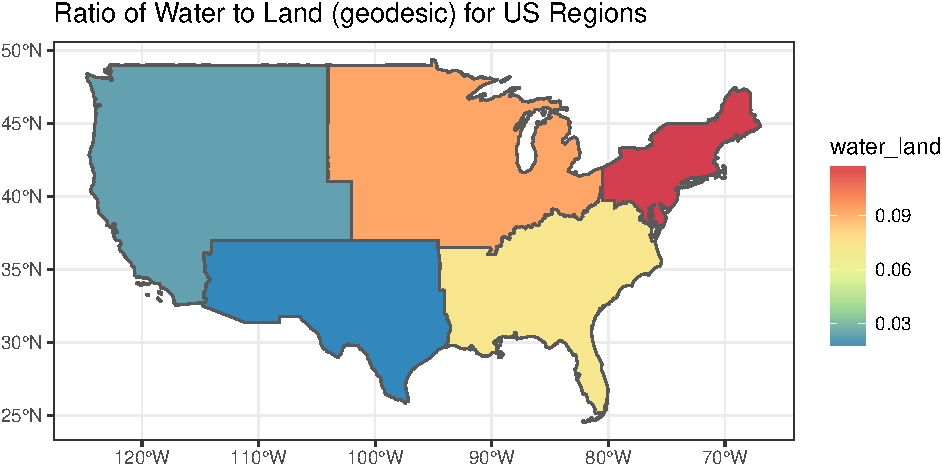
\includegraphics{R-adv-spatial_files/figure-latex/unnamed-chunk-6-1.pdf}

\section{Pipe Operator}\label{pipe-operator}

\begin{itemize}
\tightlist
\item
  Help \textgreater{} Keyboard Shortcuts Help.
\end{itemize}

\section{Challenge: Project States and Calculate
Area}\label{challenge-project-states-and-calculate-area}

Use \texttt{st\_transform()}
\href{http://spatialreference.org/ref/esri/usa-contiguous-albers-equal-area-conic/}{USA
Contiguous Albers Equal Area Conic: ESRI Projection -- Spatial
Reference}.

\subsection{Answers}\label{answers-1}

\begin{itemize}
\tightlist
\item
  ESRI:102003
\end{itemize}

\begin{Shaded}
\begin{Highlighting}[]
\KeywordTok{library}\NormalTok{(geosphere)}
\KeywordTok{library}\NormalTok{(units)}

\CommentTok{# Proj4 of http://spatialreference.org/ref/esri/usa-contiguous-albers-equal-area-conic/}
\NormalTok{crs_usa =}\StringTok{ '+proj=aea +lat_1=29.5 +lat_2=45.5 +lat_0=37.5 +lon_0=-96 +x_0=0 +y_0=0 +ellps=GRS80 +datum=NAD83 +units=m +no_defs'}

\NormalTok{regions =}\StringTok{ }\NormalTok{states %>%}
\StringTok{  }\KeywordTok{st_transform}\NormalTok{(crs_usa) %>%}
\StringTok{  }\KeywordTok{mutate}\NormalTok{(}
    \DataTypeTok{water_m2 =} \NormalTok{AWATER %>%}\StringTok{ }\KeywordTok{set_units}\NormalTok{(m^}\DecValTok{2}\NormalTok{),}
    \DataTypeTok{land_m2  =} \NormalTok{geometry %>%}\StringTok{ }\KeywordTok{st_zm}\NormalTok{() %>%}\StringTok{ }\KeywordTok{st_area}\NormalTok{()) %>%}
\StringTok{  }\KeywordTok{group_by}\NormalTok{(region) %>%}
\StringTok{  }\KeywordTok{summarize}\NormalTok{(}
    \DataTypeTok{water_m2 =} \KeywordTok{sum}\NormalTok{(water_m2),}
    \DataTypeTok{land_m2  =} \KeywordTok{sum}\NormalTok{(land_m2)) %>%}
\StringTok{  }\KeywordTok{mutate}\NormalTok{(}
    \DataTypeTok{water_land =} \NormalTok{water_m2 /}\StringTok{ }\NormalTok{land_m2)}

\CommentTok{# table}
\NormalTok{regions %>%}
\StringTok{  }\KeywordTok{st_set_geometry}\NormalTok{(}\OtherTok{NULL}\NormalTok{) %>%}
\StringTok{  }\KeywordTok{arrange}\NormalTok{(}\KeywordTok{desc}\NormalTok{(water_land))}
\end{Highlighting}
\end{Shaded}

\begin{verbatim}
## # A tibble: 5 x 4
##      region         water_m2          land_m2   water_land
##       <chr>          <units>          <units>      <units>
## 1 Northeast 108922434345 m^2 9.117031e+11 m^2 0.11947138 1
## 2   Midwest 184383393833 m^2 1.987266e+12 m^2 0.09278246 1
## 3 Southeast 103876652998 m^2 1.427078e+12 m^2 0.07278973 1
## 4      West  57568049509 m^2 2.467167e+12 m^2 0.02333367 1
## 5 Southwest  24217682268 m^2 1.483758e+12 m^2 0.01632185 1
\end{verbatim}

\begin{Shaded}
\begin{Highlighting}[]
\CommentTok{# plot, ggplot}
\KeywordTok{ggplot}\NormalTok{(regions) +}
\StringTok{  }\KeywordTok{geom_sf}\NormalTok{(}\KeywordTok{aes}\NormalTok{(}\DataTypeTok{fill =} \KeywordTok{as.numeric}\NormalTok{(water_land))) +}
\StringTok{  }\KeywordTok{scale_fill_distiller}\NormalTok{(}\StringTok{"water_land"}\NormalTok{, }\DataTypeTok{palette =} \StringTok{"Spectral"}\NormalTok{) +}
\StringTok{  }\KeywordTok{theme_bw}\NormalTok{() +}
\StringTok{  }\KeywordTok{ggtitle}\NormalTok{(}\StringTok{"Ratio of Water to Land (geodesic) for US Regions "}\NormalTok{)}
\end{Highlighting}
\end{Shaded}

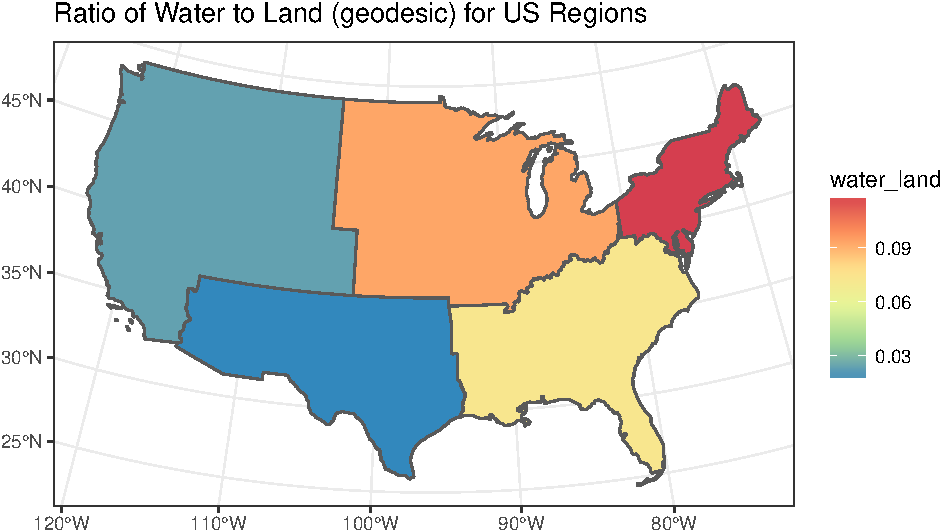
\includegraphics{R-adv-spatial_files/figure-latex/unnamed-chunk-7-1.pdf}

\section{Key Points}\label{key-points}

\begin{itemize}
\tightlist
\item
  Area can be calculated a variety of ways. Geodesic is preferred if
  starting with geographic coordinates (vs projected).
\end{itemize}

\section{Issues}\label{issues}

\begin{itemize}
\tightlist
\item
  \texttt{sf::st\_is\_valid()}
\end{itemize}

\chapter{Interactive Maps}\label{interactive}

Resources:

\begin{itemize}
\tightlist
\item
  \href{http://remi-daigle.github.io/2016-04-15-UCSB/viz/}{Visualization
  in R}
\item
  \href{http://rstudio.github.io/leaflet/}{Leaflet for R - Introduction}
\item
  \href{http://r-spatial.org/r/2017/01/30/mapedit_intro.html}{mapedit -
  interactively edit spatial data in R}
\item
  \href{https://r-spatial.github.io/mapview/}{Interactive Viewing of
  Spatial Objects in R • mapview}
\end{itemize}

\section{Overview}\label{overview-1}

\textbf{Questions} - How do you generate interactive plots of spatial
data?

\section{\texorpdfstring{\textbf{Objectives}}{Objectives}}\label{objectives}

\section{Things You'll Need to Complete this
Tutorial}\label{things-youll-need-to-complete-this-tutorial-1}

\textbf{R Skill Level}: Intermediate - you've got basics of R down.

You'll need \ldots{}

We will continue to use the \texttt{sf} and \texttt{raster} packages and
introduce the \texttt{leaflet} package in this tutorial.

\begin{Shaded}
\begin{Highlighting}[]
\CommentTok{# load packages}
\KeywordTok{library}\NormalTok{(tidyverse)  }\CommentTok{# loads dplyr, tidyr, ggplot2 packages}
\KeywordTok{library}\NormalTok{(sf)         }\CommentTok{# simple features package - vector}
\KeywordTok{library}\NormalTok{(raster)     }\CommentTok{# raster}
\KeywordTok{library}\NormalTok{(leaflet)    }\CommentTok{# interactive}

\CommentTok{# set working directory to data folder}
\CommentTok{# setwd("pathToDirHere")}
\end{Highlighting}
\end{Shaded}

\section{States: ggplot2}\label{states-ggplot2}

\begin{Shaded}
\begin{Highlighting}[]
\CommentTok{# read in states}
\NormalTok{states <-}\StringTok{ }\KeywordTok{read_sf}\NormalTok{(}\StringTok{"data/NEON-DS-Site-Layout-Files/US-Boundary-Layers/US-State-Boundaries-Census-2014.shp"}\NormalTok{) %>%}
\StringTok{  }\KeywordTok{st_zm}\NormalTok{() %>%}
\StringTok{  }\KeywordTok{mutate}\NormalTok{(}
    \DataTypeTok{water_km2 =} \NormalTok{(AWATER /}\StringTok{ }\NormalTok{(}\DecValTok{1000}\NormalTok{*}\DecValTok{1000}\NormalTok{)) %>%}\StringTok{ }\KeywordTok{round}\NormalTok{(}\DecValTok{1}\NormalTok{))}

\CommentTok{# plot, ggplot}
\NormalTok{g =}\StringTok{ }\KeywordTok{ggplot}\NormalTok{(states) +}
\StringTok{  }\KeywordTok{geom_sf}\NormalTok{(}\KeywordTok{aes}\NormalTok{(}\DataTypeTok{fill =} \NormalTok{water_km2)) +}
\StringTok{  }\KeywordTok{scale_fill_distiller}\NormalTok{(}\StringTok{"water_land"}\NormalTok{, }\DataTypeTok{palette =} \StringTok{"Spectral"}\NormalTok{) +}
\StringTok{  }\KeywordTok{ggtitle}\NormalTok{(}\StringTok{"Amount of Water by State"}\NormalTok{)}
\NormalTok{g}
\end{Highlighting}
\end{Shaded}

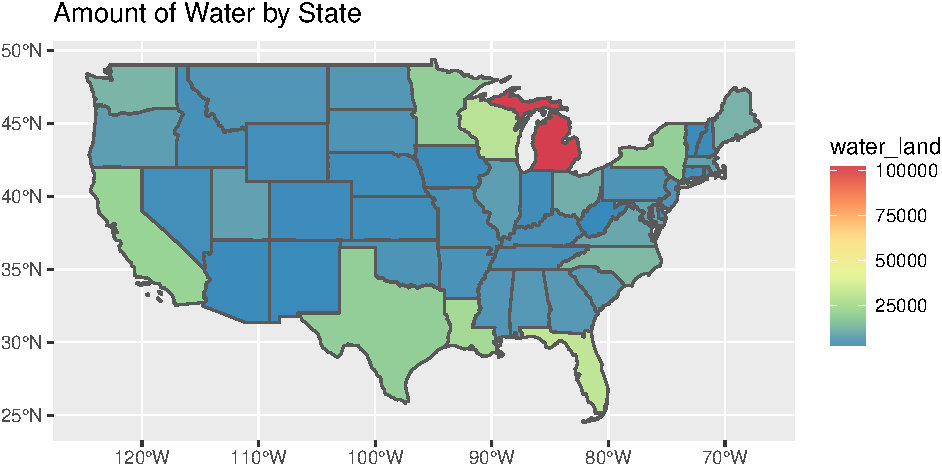
\includegraphics{R-adv-spatial_files/figure-latex/unnamed-chunk-10-1.pdf}

\section{States: plotly}\label{states-plotly}

\begin{Shaded}
\begin{Highlighting}[]
\KeywordTok{library}\NormalTok{(plotly)}

\KeywordTok{ggplotly}\NormalTok{(g)}
\end{Highlighting}
\end{Shaded}

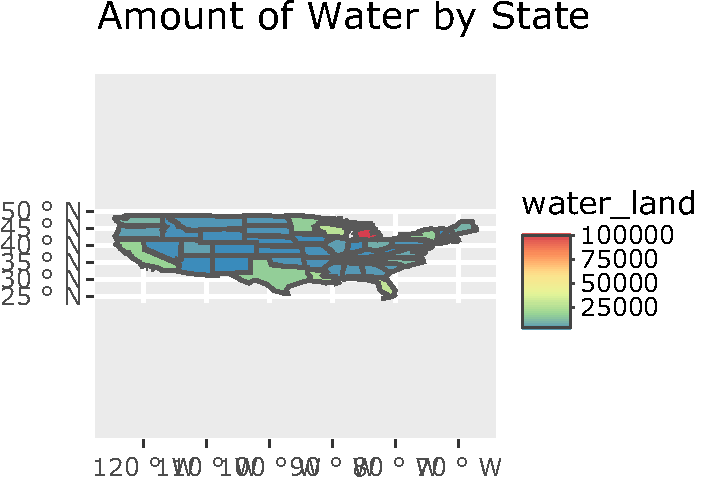
\includegraphics{R-adv-spatial_files/figure-latex/unnamed-chunk-11-1.pdf}

\section{States: mapview}\label{states-mapview}

\begin{Shaded}
\begin{Highlighting}[]
\KeywordTok{library}\NormalTok{(mapview)}

\KeywordTok{mapview}\NormalTok{(states)}
\end{Highlighting}
\end{Shaded}

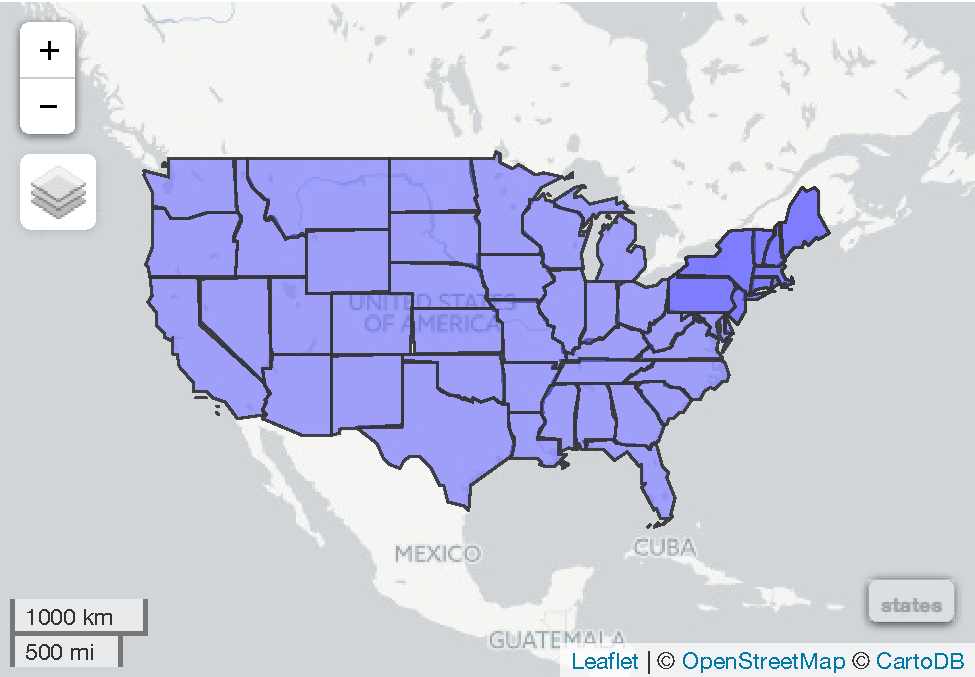
\includegraphics{R-adv-spatial_files/figure-latex/unnamed-chunk-12-1.pdf}

\begin{Shaded}
\begin{Highlighting}[]
\KeywordTok{mapview}\NormalTok{(states, }\DataTypeTok{zcol=}\StringTok{'water_km2'}\NormalTok{, }\DataTypeTok{burst=}\StringTok{'STUSPS'}\NormalTok{) }\CommentTok{# , burst = TRUE, hide = TRUE) # , burst=T)}
\end{Highlighting}
\end{Shaded}

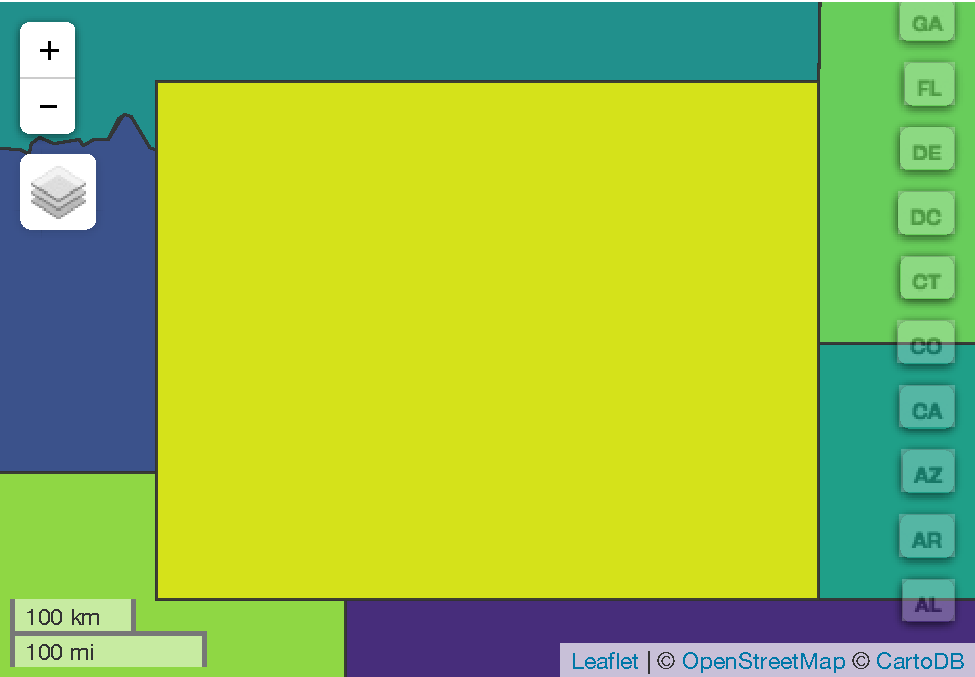
\includegraphics{R-adv-spatial_files/figure-latex/unnamed-chunk-12-2.pdf}

\section{States: leaflet}\label{states-leaflet}

\begin{Shaded}
\begin{Highlighting}[]
\KeywordTok{library}\NormalTok{(leaflet)}

\KeywordTok{leaflet}\NormalTok{(states) %>%}
\StringTok{  }\KeywordTok{addTiles}\NormalTok{() %>%}
\StringTok{  }\KeywordTok{addPolygons}\NormalTok{()}
\end{Highlighting}
\end{Shaded}

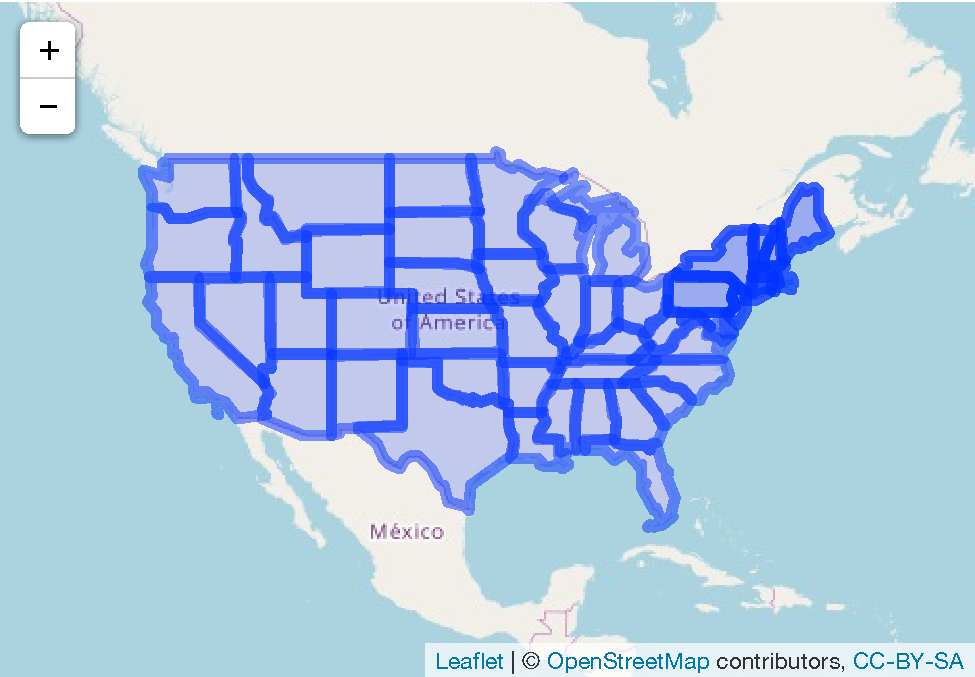
\includegraphics{R-adv-spatial_files/figure-latex/unnamed-chunk-13-1.pdf}

\subsection{Choropleth}\label{choropleth}

\begin{itemize}
\tightlist
\item
  \href{http://rstudio.github.io/leaflet/choropleths.html}{Leaflet for R
  - Choropleths}
\end{itemize}

\begin{Shaded}
\begin{Highlighting}[]
\NormalTok{pal <-}\StringTok{ }\KeywordTok{colorBin}\NormalTok{(}\StringTok{"Blues"}\NormalTok{, }\DataTypeTok{domain =} \NormalTok{states$water_km2, }\DataTypeTok{bins =} \DecValTok{7}\NormalTok{)}


\KeywordTok{leaflet}\NormalTok{(states) %>%}
\StringTok{  }\KeywordTok{addProviderTiles}\NormalTok{(}\StringTok{"Stamen.TonerLite"}\NormalTok{) %>%}
\StringTok{  }\KeywordTok{addPolygons}\NormalTok{(}
    \CommentTok{# fill}
    \DataTypeTok{fillColor   =} \NormalTok{~}\KeywordTok{pal}\NormalTok{(water_km2),}
    \DataTypeTok{fillOpacity =} \FloatTok{0.7}\NormalTok{,}
    \CommentTok{# line}
    \DataTypeTok{dashArray   =} \StringTok{"3"}\NormalTok{,}
    \DataTypeTok{weight      =} \DecValTok{2}\NormalTok{,}
    \DataTypeTok{color       =} \StringTok{"white"}\NormalTok{,}
    \DataTypeTok{opacity     =} \DecValTok{1}\NormalTok{,}
    \CommentTok{# interaction}
    \DataTypeTok{highlight =} \KeywordTok{highlightOptions}\NormalTok{(}
      \DataTypeTok{weight =} \DecValTok{5}\NormalTok{,}
      \DataTypeTok{color =} \StringTok{"#666"}\NormalTok{,}
      \DataTypeTok{dashArray =} \StringTok{""}\NormalTok{,}
      \DataTypeTok{fillOpacity =} \FloatTok{0.7}\NormalTok{,}
      \DataTypeTok{bringToFront =} \OtherTok{TRUE}\NormalTok{))}
\end{Highlighting}
\end{Shaded}

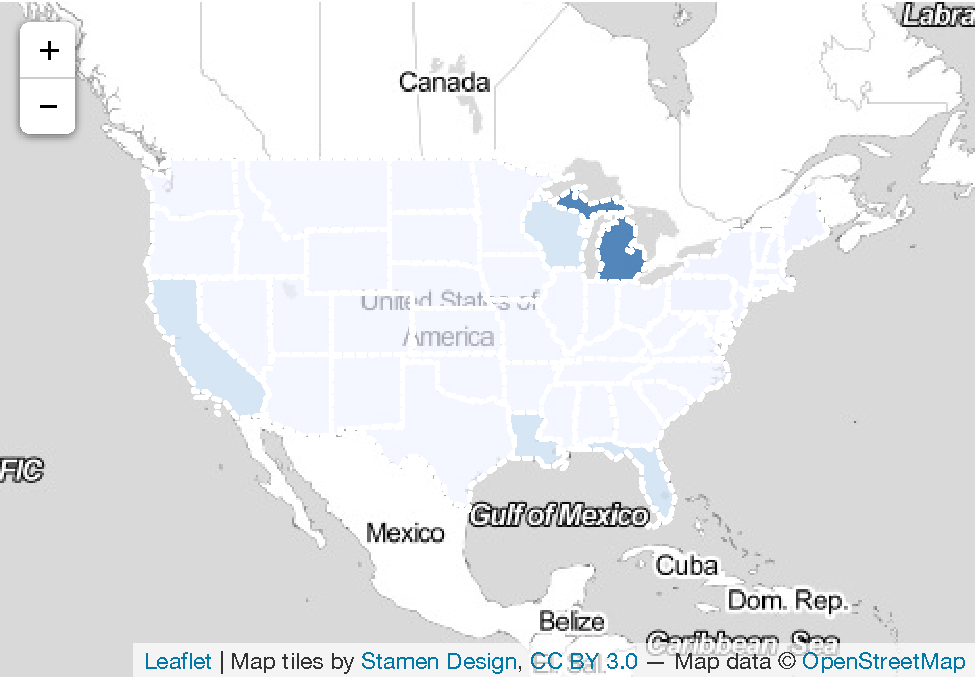
\includegraphics{R-adv-spatial_files/figure-latex/unnamed-chunk-14-1.pdf}

\subsection{Popups and Legend}\label{popups-and-legend}

\begin{Shaded}
\begin{Highlighting}[]
\KeywordTok{library}\NormalTok{(htmltools)}
\KeywordTok{library}\NormalTok{(scales)}

\NormalTok{labels <-}\StringTok{ }\KeywordTok{sprintf}\NormalTok{(}
  \StringTok{"<strong>%s</strong><br/> water: %s km<sup>2</sup>"}\NormalTok{,}
  \NormalTok{states$NAME, }\KeywordTok{comma}\NormalTok{(states$water_km2)) %>%}\StringTok{ }
\StringTok{  }\KeywordTok{lapply}\NormalTok{(HTML)}

\KeywordTok{leaflet}\NormalTok{(states) %>%}
\StringTok{  }\KeywordTok{addProviderTiles}\NormalTok{(}\StringTok{"Stamen.TonerLite"}\NormalTok{) %>%}
\StringTok{  }\KeywordTok{addPolygons}\NormalTok{(}
    \CommentTok{# fill}
    \DataTypeTok{fillColor   =} \NormalTok{~}\KeywordTok{pal}\NormalTok{(water_km2),}
    \DataTypeTok{fillOpacity =} \FloatTok{0.7}\NormalTok{,}
    \CommentTok{# line}
    \DataTypeTok{dashArray   =} \StringTok{"3"}\NormalTok{,}
    \DataTypeTok{weight      =} \DecValTok{2}\NormalTok{,}
    \DataTypeTok{color       =} \StringTok{"white"}\NormalTok{,}
    \DataTypeTok{opacity     =} \DecValTok{1}\NormalTok{,}
    \CommentTok{# interaction}
    \DataTypeTok{highlight =} \KeywordTok{highlightOptions}\NormalTok{(}
      \DataTypeTok{weight =} \DecValTok{5}\NormalTok{,}
      \DataTypeTok{color =} \StringTok{"#666"}\NormalTok{,}
      \DataTypeTok{dashArray =} \StringTok{""}\NormalTok{,}
      \DataTypeTok{fillOpacity =} \FloatTok{0.7}\NormalTok{,}
      \DataTypeTok{bringToFront =} \OtherTok{TRUE}\NormalTok{),}
  \DataTypeTok{label =} \NormalTok{labels,}
  \DataTypeTok{labelOptions =} \KeywordTok{labelOptions}\NormalTok{(}
    \DataTypeTok{style =} \KeywordTok{list}\NormalTok{(}\StringTok{"font-weight"} \NormalTok{=}\StringTok{ "normal"}\NormalTok{, }\DataTypeTok{padding =} \StringTok{"3px 8px"}\NormalTok{),}
    \DataTypeTok{textsize =} \StringTok{"15px"}\NormalTok{,}
    \DataTypeTok{direction =} \StringTok{"auto"}\NormalTok{)) %>%}
\StringTok{  }\KeywordTok{addLegend}\NormalTok{(}
    \DataTypeTok{pal =} \NormalTok{pal, }\DataTypeTok{values =} \NormalTok{~water_km2, }\DataTypeTok{opacity =} \FloatTok{0.7}\NormalTok{, }\DataTypeTok{title =} \KeywordTok{HTML}\NormalTok{(}\StringTok{"Water (km<sup>2</sup>)"}\NormalTok{),}
    \DataTypeTok{position =} \StringTok{"bottomright"}\NormalTok{)}
\end{Highlighting}
\end{Shaded}

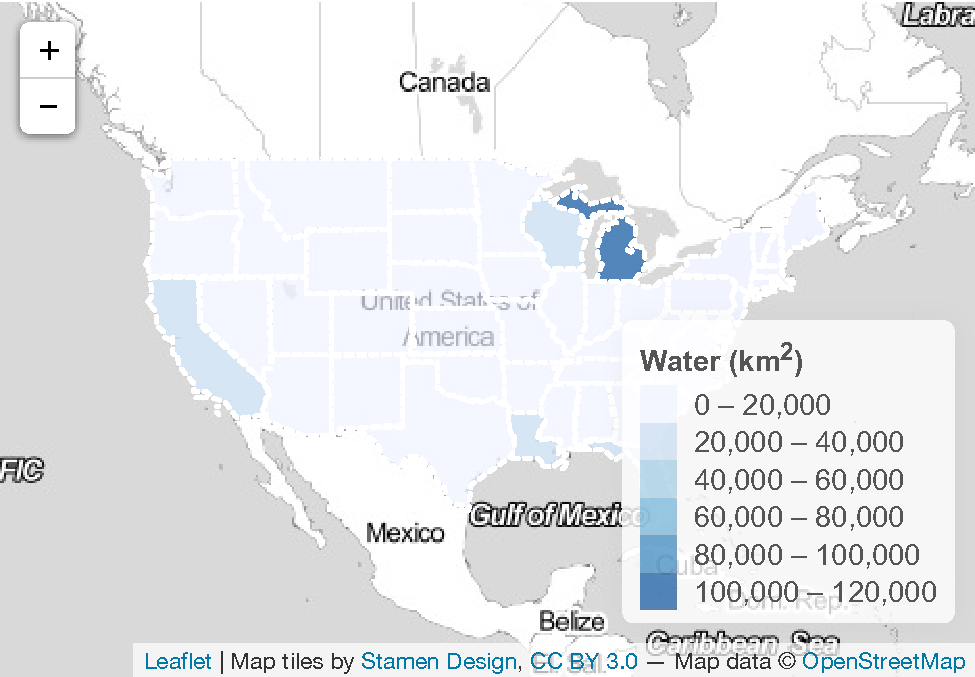
\includegraphics{R-adv-spatial_files/figure-latex/unnamed-chunk-15-1.pdf}

\section{Pipe Operator}\label{pipe-operator-1}

\begin{itemize}
\tightlist
\item
  Help \textgreater{} Keyboard Shortcuts Help.
\end{itemize}

\section{Challenge: Project States and Calculate
Area}\label{challenge-project-states-and-calculate-area-1}

Use \texttt{st\_transform()}
\href{http://spatialreference.org/ref/esri/usa-contiguous-albers-equal-area-conic/}{USA
Contiguous Albers Equal Area Conic: ESRI Projection -- Spatial
Reference}.

\subsection{Answers}\label{answers-2}

\begin{itemize}
\tightlist
\item
  ESRI:102003
\end{itemize}

\begin{Shaded}
\begin{Highlighting}[]
\KeywordTok{library}\NormalTok{(geosphere)}
\KeywordTok{library}\NormalTok{(units)}

\CommentTok{# Proj4 of http://spatialreference.org/ref/esri/usa-contiguous-albers-equal-area-conic/}
\NormalTok{crs_usa =}\StringTok{ '+proj=aea +lat_1=29.5 +lat_2=45.5 +lat_0=37.5 +lon_0=-96 +x_0=0 +y_0=0 +ellps=GRS80 +datum=NAD83 +units=m +no_defs'}

\NormalTok{regions =}\StringTok{ }\NormalTok{states %>%}
\StringTok{  }\KeywordTok{st_transform}\NormalTok{(crs_usa) %>%}
\StringTok{  }\KeywordTok{mutate}\NormalTok{(}
    \DataTypeTok{water_m2 =} \NormalTok{water_km2 %>%}\StringTok{ }\KeywordTok{set_units}\NormalTok{(m^}\DecValTok{2}\NormalTok{),}
    \DataTypeTok{land_m2  =} \NormalTok{geometry %>%}\StringTok{ }\KeywordTok{st_zm}\NormalTok{() %>%}\StringTok{ }\KeywordTok{st_area}\NormalTok{()) %>%}
\StringTok{  }\KeywordTok{group_by}\NormalTok{(region) %>%}
\StringTok{  }\KeywordTok{summarize}\NormalTok{(}
    \DataTypeTok{water_m2 =} \KeywordTok{sum}\NormalTok{(water_m2),}
    \DataTypeTok{land_m2  =} \KeywordTok{sum}\NormalTok{(land_m2)) %>%}
\StringTok{  }\KeywordTok{mutate}\NormalTok{(}
    \DataTypeTok{water_land =} \NormalTok{water_m2 /}\StringTok{ }\NormalTok{land_m2)}

\CommentTok{# table}
\NormalTok{regions %>%}
\StringTok{  }\KeywordTok{st_set_geometry}\NormalTok{(}\OtherTok{NULL}\NormalTok{) %>%}
\StringTok{  }\KeywordTok{arrange}\NormalTok{(}\KeywordTok{desc}\NormalTok{(water_land))}
\end{Highlighting}
\end{Shaded}

\begin{verbatim}
## # A tibble: 5 x 4
##      region     water_m2          land_m2     water_land
##       <chr>      <units>          <units>        <units>
## 1 Northeast 108922.9 m^2 9.117031e+11 m^2 1.194719e-07 1
## 2   Midwest 184383.2 m^2 1.987266e+12 m^2 9.278237e-08 1
## 3 Southeast 103876.6 m^2 1.427078e+12 m^2 7.278970e-08 1
## 4      West  57568.0 m^2 2.467167e+12 m^2 2.333365e-08 1
## 5 Southwest  24217.7 m^2 1.483758e+12 m^2 1.632186e-08 1
\end{verbatim}

\begin{Shaded}
\begin{Highlighting}[]
\CommentTok{# plot, ggplot}
\KeywordTok{ggplot}\NormalTok{(regions) +}
\StringTok{  }\KeywordTok{geom_sf}\NormalTok{(}\KeywordTok{aes}\NormalTok{(}\DataTypeTok{fill =} \KeywordTok{as.numeric}\NormalTok{(water_land))) +}
\StringTok{  }\KeywordTok{scale_fill_distiller}\NormalTok{(}\StringTok{"water_land"}\NormalTok{, }\DataTypeTok{palette =} \StringTok{"Spectral"}\NormalTok{) +}
\StringTok{  }\KeywordTok{theme_bw}\NormalTok{() +}
\StringTok{  }\KeywordTok{ggtitle}\NormalTok{(}\StringTok{"Ratio of Water to Land (geodesic) for US Regions "}\NormalTok{)}
\end{Highlighting}
\end{Shaded}

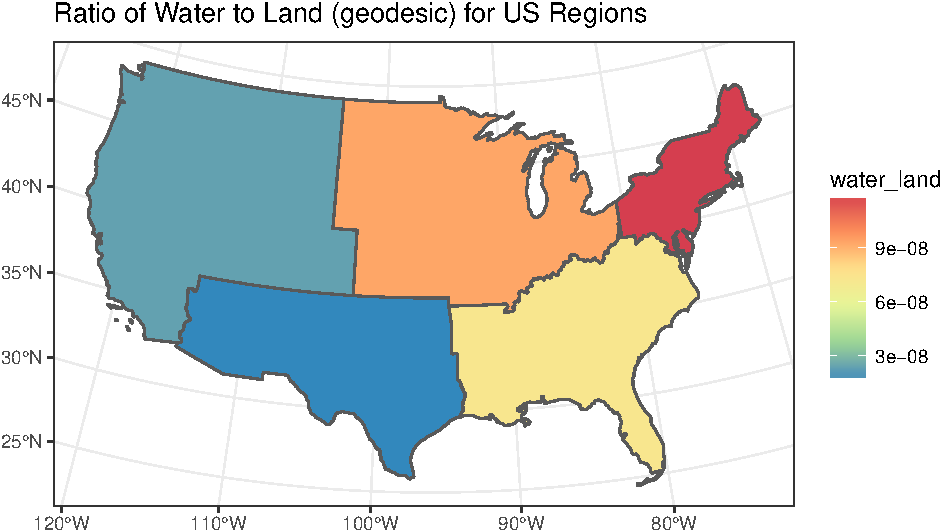
\includegraphics{R-adv-spatial_files/figure-latex/unnamed-chunk-16-1.pdf}

\section{Key Points}\label{key-points-1}

\begin{itemize}
\tightlist
\item
  Area can be calculated a variety of ways. Geodesic is preferred if
  starting with geographic coordinates (vs projected).
\end{itemize}

\section{Issues}\label{issues-1}

\begin{itemize}
\tightlist
\item
  \texttt{sf::st\_is\_valid()}
\end{itemize}


\end{document}
